\documentclass[12pt]{article}

\usepackage{amsmath}
\usepackage{array}
\usepackage{caption}
\usepackage[top=1in, bottom=1in, left=0.75in, right=0.75in]{geometry}
\usepackage{graphicx}
\usepackage[colorlinks=true, allcolors=blue]{hyperref}
\usepackage[utf8]{inputenc}
\usepackage{multirow}
\usepackage{pdfpages}
\usepackage[section]{placeins}

\graphicspath{{figures/}}

\begin{document}

\begin{titlepage}
  \begin{center} \LARGE
    \vspace*{1.5in}

    ECE 272 Pre-Lab 3

    Fall 2018

    \vfill

    Combinational Logic (Seven Segment Driver)

    Phi Luu

    \vfill

    October 8\textsuperscript{th}, 2018

    Grading TA: Edgar Perez

    \vspace{1.5in}
  \end{center}
\end{titlepage}

{\Large Design a 7 segment display decoder.}

\rule{0em}{1.5em}

A seven-segment display is an electronic device that uses seven LEDs to display decimal digits (0 - 9). The seven segments are arranged like an italic 8 and have an alphabetical order, as illustrated by Figure~\ref{figure:1} below:

\begin{figure}[h]
  \centering
  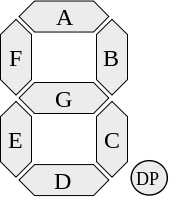
\includegraphics[width=0.25\textwidth]{seven_segment_diplay.png}
  \caption{The LED segments and their order in a seven-segment display. \href{https://commons.wikimedia.org/wiki/Seven_segment_display}{Source}}
  \label{figure:1}
\end{figure}

Depending on the input (0 - 9), some LEDs will turn on or off to form a pattern that illustrates the according decimal digit. Based on this concept, the input (0 - 9) can be represented as a 4-bit binary number---as circuits, logic, and computers operate in binary. The decimal digit patterns of the seven-segment display are as in Figure~\ref{figure:2} below:

\begin{figure}[h]
  \centering
  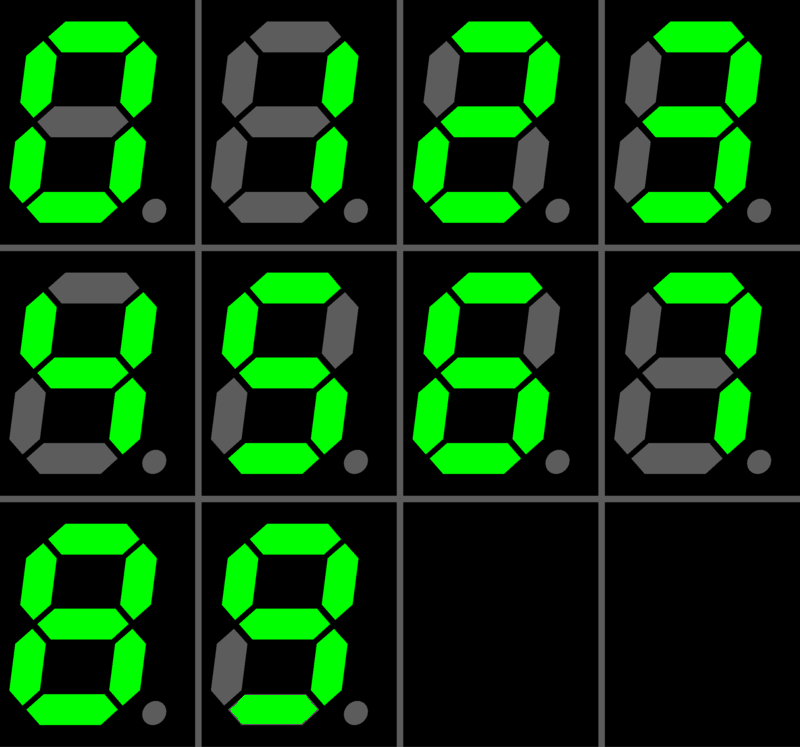
\includegraphics[width=0.35\textwidth]{seven_segment_decimal_digits.png}
  \caption{Decimal digits illustrated by a seven-segment display. \href{https://commons.wikimedia.org/wiki/Seven_segment_display}{Source}}
  \label{figure:2}
\end{figure}

Based on these concepts, a truth table converting 4-bit binary numbers to decimal digits on a seven-segment display is shown in Table~\ref{table:3}.

\newpage

\begin{table}[h]
  \centering
  \begin{tabular}{ | c | c | c | c | c || c | c | c | c | c | c | c | }
  \hline
  \multirow{2}{*}{\textbf{Digit}} & \multicolumn{4}{c||}{\textbf{4-bit input}}        & \multicolumn{7}{c|}{\textbf{7-segment output}}                                           \\ \cline{2-12}
                  & \textbf{A} & \textbf{B} & \textbf{C} & \textbf{D} & \textbf{a} & \textbf{b} & \textbf{c} & \textbf{d} & \textbf{e} & \textbf{f} & \textbf{g} \\ \hline
  \textbf{0}                      & 0          & 0          & 0          & 0          & 1          & 1          & 1          & 1          & 1          & 1          & 0          \\ \hline
  \textbf{1}                      & 0          & 0          & 0          & 1          & 0          & 1          & 1          & 0          & 0          & 0          & 0          \\ \hline
  \textbf{2}                      & 0          & 0          & 1          & 0          & 1          & 1          & 0          & 1          & 1          & 0          & 1          \\ \hline
  \textbf{3}                      & 0          & 0          & 1          & 1          & 1          & 1          & 1          & 1          & 0          & 0          & 1          \\ \hline
  \textbf{4}                      & 0          & 1          & 0          & 0          & 0          & 1          & 1          & 0          & 0          & 1          & 1          \\ \hline
  \textbf{5}                      & 0          & 1          & 0          & 1          & 1          & 0          & 1          & 1          & 0          & 1          & 1          \\ \hline
  \textbf{6}                      & 0          & 1          & 1          & 0          & 1          & 0          & 1          & 1          & 1          & 1          & 1          \\ \hline
  \textbf{7}                      & 0          & 1          & 1          & 1          & 1          & 1          & 1          & 0          & 0          & 0          & 0          \\ \hline
  \textbf{8}                      & 1          & 0          & 0          & 0          & 1          & 1          & 1          & 1          & 1          & 1          & 1          \\ \hline
  \textbf{9}                      & 1          & 0          & 0          & 1          & 1          & 1          & 1          & 1          & 0          & 1          & 1          \\ \hline
  \end{tabular}
  \caption{Truth table showing decimal digits' 4-bit binary inputs and their corresponding 7-segment outputs}
  \label{table:1}
\end{table}

To better grasp the layout of the input, output, and the decoder, the block diagrams of the seven-segment display is shown in Figure~\ref{figure:3} below:

\begin{figure}[h]
  \centering
  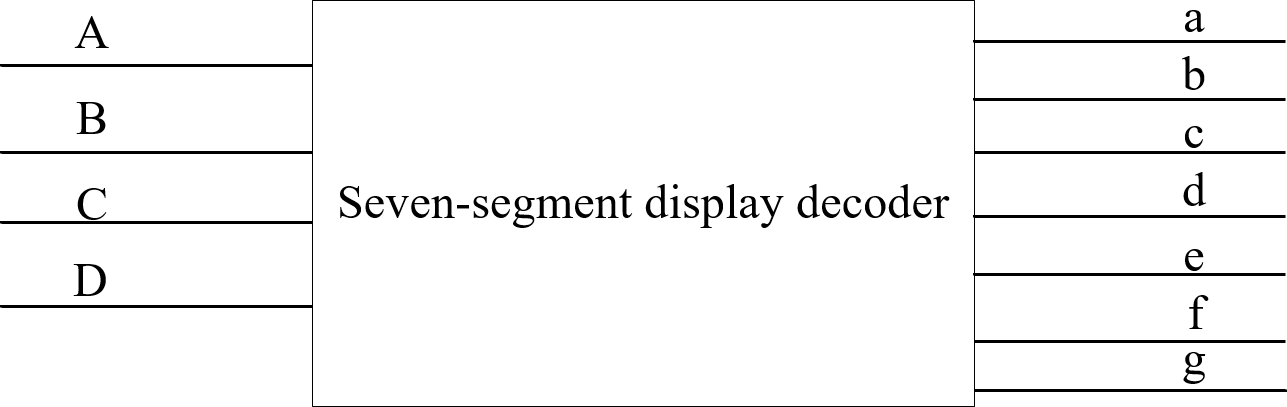
\includegraphics[width=0.75\textwidth]{seven_segment_display_block_diagram.png}
  \caption{The block diagram of the design}
  \label{figure:3}
\end{figure}

Since the device is a decoder, it asserts exactly one of its outputs depending on the input combination. Based on Table~\ref{table:1}, the following Karnaugh maps are constructed:

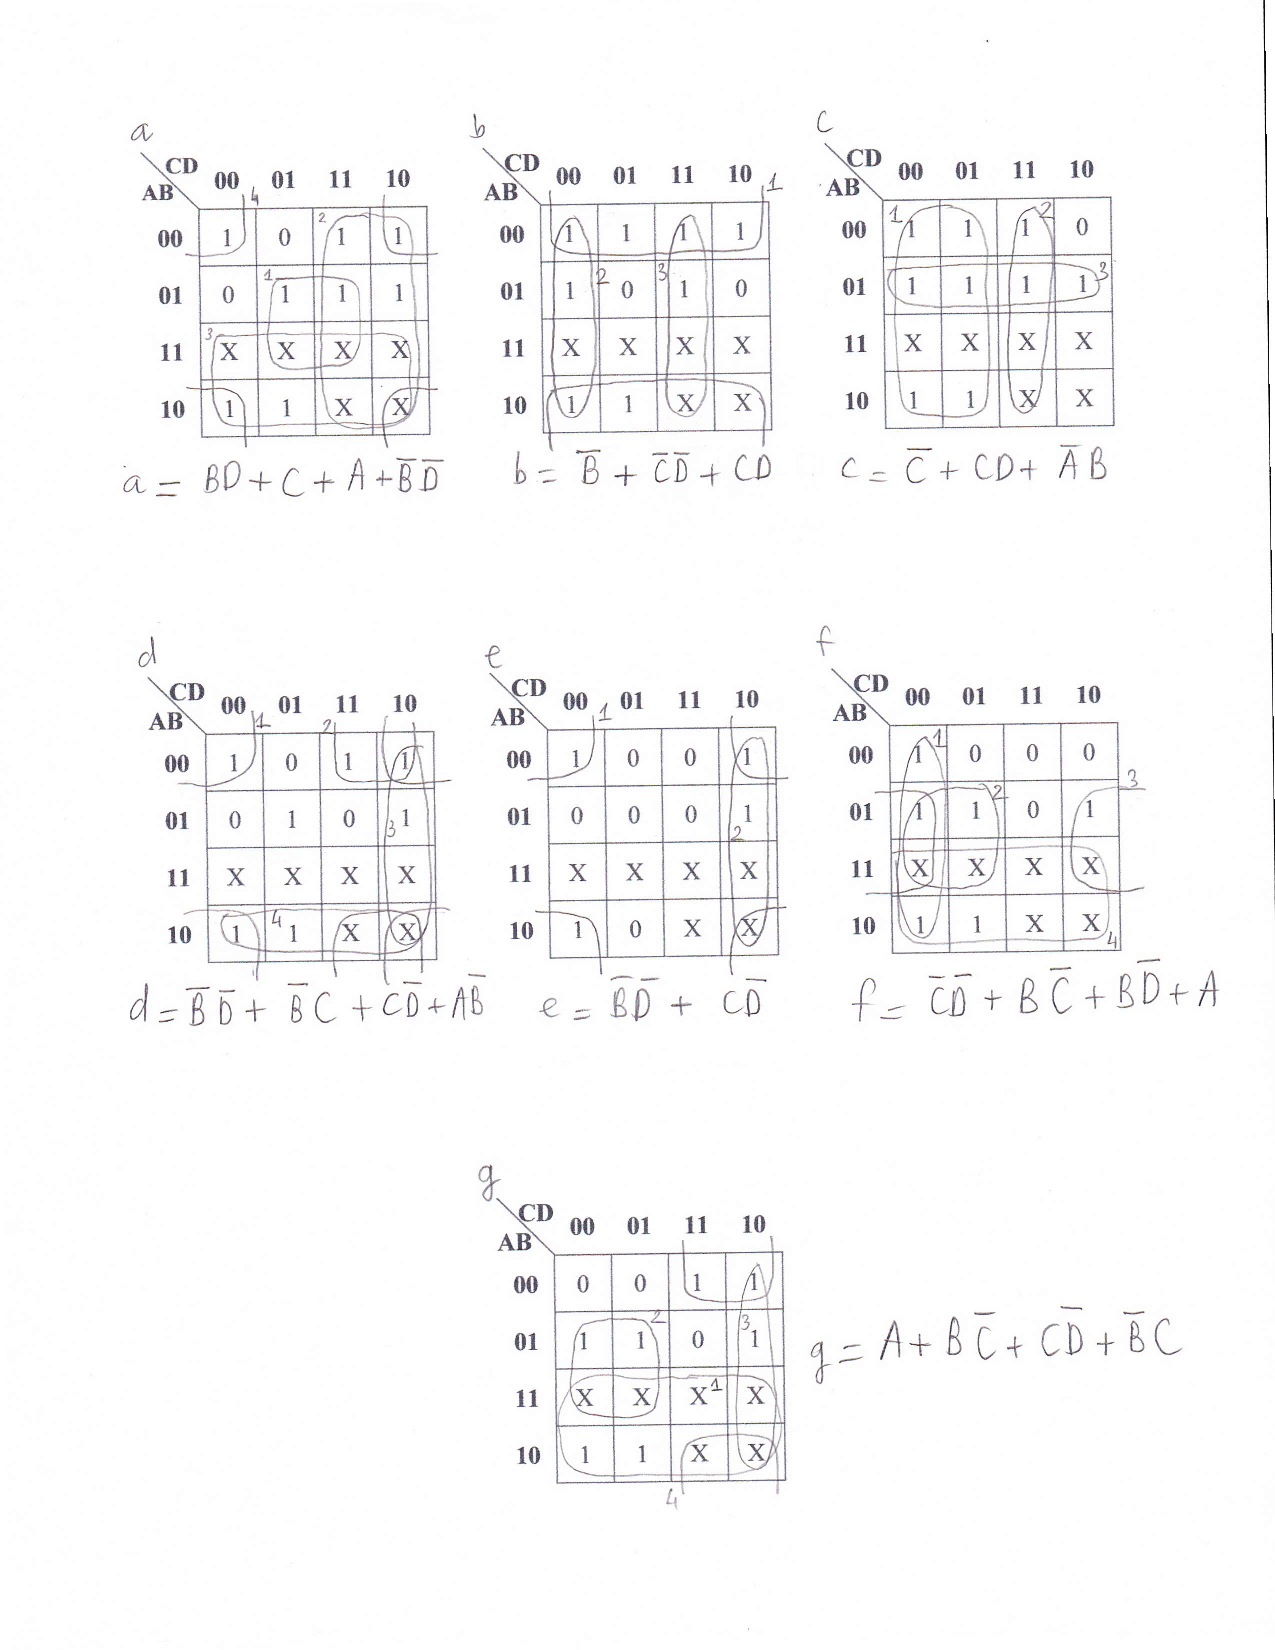
\includepdf[page=-]{seven_segments_karnaugh_map}

Based on these maps,

\begin{equation} \label{equation:1}
  a = BD + C + A + \bar{B}\bar{D}
\end{equation}

\begin{equation} \label{equation:2}
  b = \bar{B} + \bar{C}\bar{D} + CD
\end{equation}

\begin{equation} \label{equation:3}
  c = \bar{C} + CD + \bar{A}B
\end{equation}

\begin{equation} \label{equation:4}
  d = \bar{B}\bar{D} + \bar{B}C + C\bar{D} + A\bar{B}
\end{equation}

\begin{equation} \label{equation:5}
  e = \bar{B}\bar{D} + C\bar{D}
\end{equation}

\begin{equation} \label{equation:6}
  f = \bar{C}\bar{D} + B\bar{C} + B\bar{D} + A
\end{equation}

\begin{equation} \label{equation:7}
  g = A + B\bar{C} + C\bar{D} + \bar{B}C
\end{equation}

Using the simplified Boolean equation of $a$, $b$, $c$, and $d$, a schematic of the seven-segment display is as in Figure~\ref{figure:4}.

\begin{figure}
  \centering
  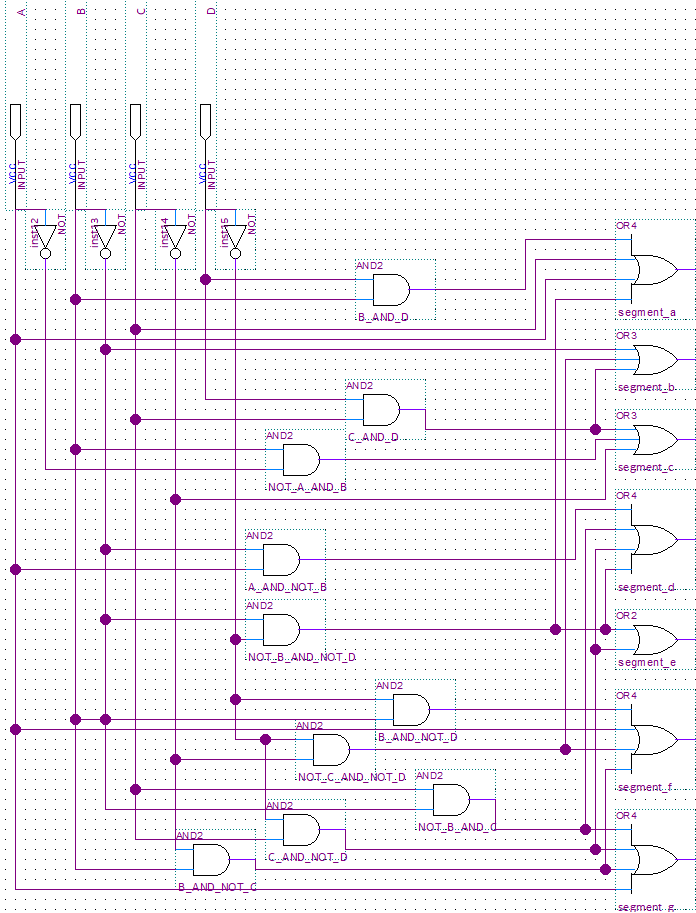
\includegraphics[width=\textwidth,height=\textheight,keepaspectratio]{seven_segment_display_schematic.png}
  \caption{A schematic design of a seven-segment display. Due to limit of space, output pins were not illustrated.}
  \label{figure:4}
\end{figure}

\end{document}
